\documentclass{article}

\usepackage{graphicx}
\usepackage[margin=2cm,a4paper]{geometry}
\usepackage{tcolorbox}
\tcbuselibrary{listings,skins}
\usepackage{microtype}
\usepackage[htt]{hyphenat}
\usepackage{placeins}
\usepackage{parskip}
\usepackage{listings}
\lstset{
  language=bash,
  basicstyle=\small\ttfamily,
  columns=flexible,
  breaklines=true,
  showstringspaces=false,
  frame=single
}

\begin{document}

\title{Building IaaS infrastructures on the AWS Cloud}
\author{Saul Pierotti}
\date{\today}

\maketitle

\section{Creation of an HTCondor Cluster for the Alignment of NGS Reads}
The demonstrative IaaS infrastructure described in this project consists of an HTCondor cluster of three nodes.
One of them acts as Master Node and the remaining two nodes as Worker Nodes.
The infrastructure is easily expandable by replicating the Worker Node instances.
The Master Node was not used also as a Worker Node since the performance benefits and cost savings would be marginal.
Also, this avoids overloading the Master Node, on which the entire cluster depends.
Finally, I implemented a shared storage space using the distributed file system NFS (Sun Microsystems, 1984) directly attached to the Master Node but available to all the Worker Nodes.

\subsection{Initialization of the Instances on the AWS Cloud}
I used the cloud service provider Amazon Web Services (AWS, \texttt{https://aws.amazon.com/}) for this project.
Worker Nodes and the Master Node were both built on similar machines.
For the Master Node, I chose the \texttt{t2.medium} instance type with a 50 Gb SSD as root storage.
For the Worker Nodes, I chose the \texttt{t2.large} instance type with a 50 Gb SSD as root storage.
The operating system adopted for both machine types is Ubuntu Server 18.04.4 LTS.
The Master Node and the Worker Nodes were all instantiated in the same availability zone (\texttt{us-east-1a}) so that they would be able to communicate through private IPv4 addresses.
The security group for the instances was configured as follows:

\begin{figure}[!h]
    \center
    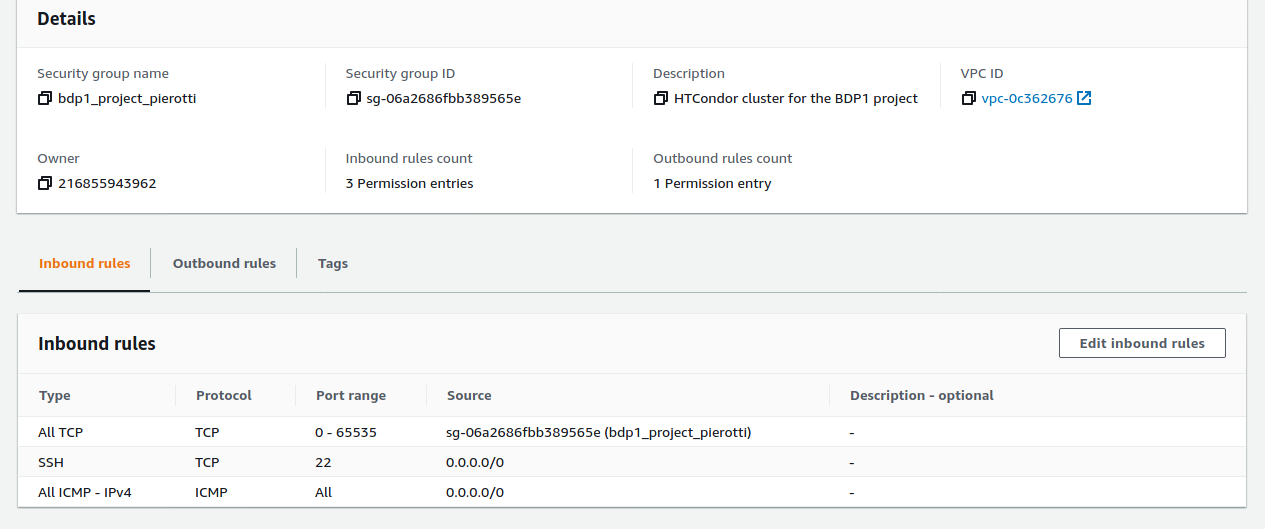
\includegraphics[width=\textwidth]{./images/security-group.png}
\end{figure}

All the TCP ports were opened to the other members of the same security group since HTCondor daemons use a dynamically assigned port.
I opened the ICMP port for accepting incoming \texttt{ping} requests for testing purposes.
Since all the TCP ports were open, there was no need for setting up additional ports for NFS.

\subsection{Configuration of the Master Node}
The PS1 prompt of the Master Node was changed so to make the node easily identifiable from the command line.

\begin{figure}[!h]
    \center
    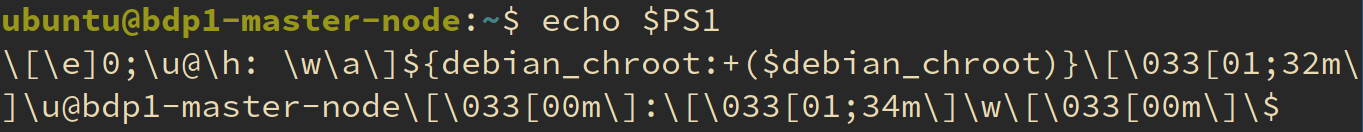
\includegraphics[width=\textwidth]{./images/master-ps1.png}
\end{figure}
\FloatBarrier

HTCondor (Thain D., Tannenbaum T., and Livny M., 2005) was then installed with the following commands:

\begin{lstlisting}
sudo su
wget -qO - https://research.cs.wisc.edu/htcondor/ubuntu/HTCondor-Release.gpg.key | apt-key add - # import the gpg key of HTCondor
echo "deb http://research.cs.wisc.edu/htcondor/ubuntu/8.8/bionic bionic contrib" >> /etc/apt/sources.list # add the repository
echo "deb-src http://research.cs.wisc.edu/htcondor/ubuntu/8.8/bionic bionic contrib" >> /etc/apt/sources.list
apt update
apt install htcondor
systemctl start condor # start and enable the condor service
systemctl enable condor
\end{lstlisting}

The correct proceeding of the installation and the start of the \texttt{condor} service where checked with the following commands:

\begin{figure}[!h]
    \center
    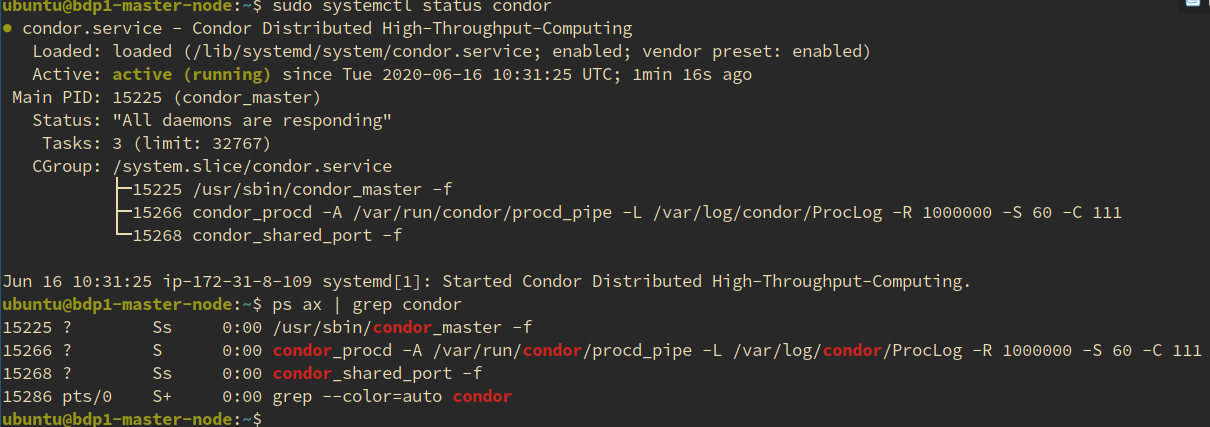
\includegraphics[width=\textwidth]{./images/condor_installed.png}
\end{figure}

The following lines where appended at the end of the main HTCondor configuration file, located at\\
\texttt{/etc/condor/condor\_config}:

\begin{lstlisting}
# Master Node IP
CONDOR_HOST = <Master_Node_private_IP>

# Master Node config 
DAEMON_LIST = COLLECTOR, MASTER, NEGOTIATOR, SCHEDD

HOSTALLOW_READ = *
HOSTALLOW_WRITE = *
HOSTALLOW_ADMINISTRATOR = *
\end{lstlisting}

Finally, the \texttt{condor} service was restarted with the following command:

\begin{lstlisting}
sudo systemctl restart condor
\end{lstlisting}

I set up the NFS server on the Master Node.
A new 100 Gb standard magnetic volume was created from the AWS interface and attached to the machine.
A primary partiton was initialized on the volume using \texttt{fdisk} and an \texttt{Ext4} file system was created onto it using \texttt{mkfs.ext4}.
The \texttt{/etc/fstab} file was modified so that the machine would mount the volume automatically at boot under the newly created directory \texttt{/data}.
The following line was appended to \texttt{/etc/fstab}:

\begin{lstlisting}
</new_volume/partiton>              /data    ext4   defaults                0 0
\end{lstlisting}

The following commands were then issued, so to install the appropriate packages:

\begin{lstlisting}
sudo apt install nfs-kernel-server
\end{lstlisting}

The following line was appended to the NFS configuration file \texttt{/etc/exports}:

\begin{lstlisting}
/data 172.31.0.0/16(rw,sync,no_wdelay)
\end{lstlisting}

Finally, I set the owner and group of the shared folder to \texttt{nobody:nogroup} and I edited the permissions of the folder so to grant unlimited access to it:

\begin{lstlisting}
sudo chown nobody:nogroup /data
sudo chmod 777 /data
\end{lstlisting}

The \texttt{/data} folder was so made available to all the Worker Nodes on the address range \texttt{172.31.0.0/16}.
This configuration does not pose a significant security risk since all the machines belong to the same Virtual Private Cloud (VPC). Only machines instantiated on the same VPC could access the exposed volume.
Moreover, this configuration grants immediate access to the volume to additional Worker Nodes instantiated in the same VPC.
I created a mock file on the \texttt{/data} folder so to be able to recognize the volume when mounted.

\begin{lstlisting}
touch /data/this_is_a_shared_NFS_volume
\end{lstlisting}

\subsection{Configuration of the Worker Nodes}
I instantiated on AWS a new t2.large machine with Ubuntu 18.04 LTS.
I changed the PS1 prompt so to make the node easily identifiable from the command line.

\begin{figure}[!h]
    \center
    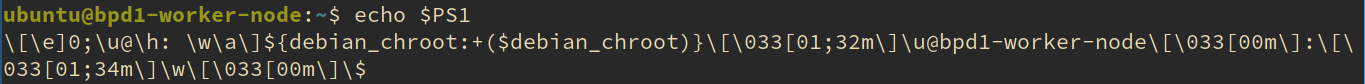
\includegraphics[width=\textwidth]{./images/worker-ps1.png}
\end{figure}

I installed HTCondor on this system with the same procedure used for the Master Node.
Only the \texttt{/etc/condor/condor\_config} file was configured differently, by appending the following lines to it:

\begin{lstlisting}
# Master Node IP
CONDOR_HOST = <Master_Node_private_IP>

# Worker Node config
DAEMON_LIST = MASTER, STARTD

HOSTALLOW_READ = *
HOSTALLOW_WRITE = *
HOSTALLOW_ADMINISTRATOR = *
\end{lstlisting}

I granted to the Worker Node access to the shared NFS volume.
The following command was issued to install the required packages:

\begin{lstlisting}
sudo apt install nfs-common
\end{lstlisting}

A new directory was then created at \texttt{/data} using the \texttt{mkdir} command.
The \texttt{/etc/fstab} file was edited by appending the following line, so that the shared volume would be automatically mounted at boot under the directory \texttt{/data}:

\begin{lstlisting}
<Master_Node_private_IP>:/data      /data    nfs    defaults                0 0
\end{lstlisting}

I verified that the shared volume was accessible from the Worker Node.

\begin{figure}[!h]
    \center
    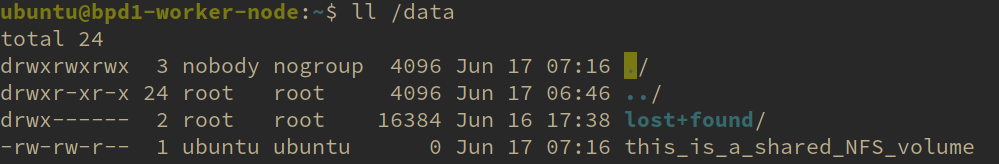
\includegraphics[width=\textwidth]{./images/nfs_works.png}
\end{figure}

I installed the application BWA on the Worker Node:

\begin{lstlisting}
sudo apt install -y bwa
\end{lstlisting}

I took a snapshot of the Worker Node virtual machine (AMI) through the AWS web interface.
In this way, the Worker Nodes could be easily replicable when more computational power would be needed.
It would be possible to deploy new Worker Nodes by simply instantiating new virtual machines from the AMI, without the need for manual configuration.

\subsection{Submission of a Test Job to the HTCondor Cluster}
I instantiated a new Worker Node from the relative AMI.
Subsequently, I created a new volume through the AWS interface from a snapshot containing test data used during the BDP1 course (\texttt{snap-09ee52d8038fb8094}, BDP1\_2020).
This snapshot contained NGS reads from 3 different patients.
Each patient had a folder with around 500 fasta files, with 1000 reads each.
The new volume was mounted on the Master Node under the directory \texttt{/data}, replacing the empty volume used before.
The \texttt{/etc/fstab} file was updated accordingly and the \texttt{nfs-server} service restarted.
Finally, I tested that the new volume was accessible from the Worker Nodes.

\begin{figure}[!h]
    \center
    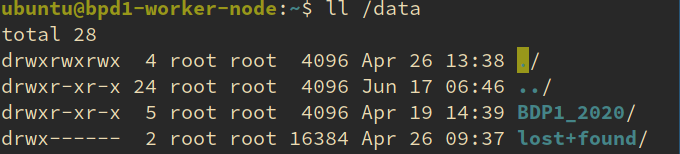
\includegraphics[width=.8\textwidth]{./images/nfs_bdp_works.png}
\end{figure}

The test job consisted in aligning ten fasta files (\texttt{read\_1.fa} to \texttt{read\_10.fa} from patient 1) to the human genome build hg19, also stored on the shared volume.
I used the BWA alignment tool (Li H. and Durbin R. 2009) for the scope.
This tool takes advantage of indexing the genome for speeding up the alignment of low-divergent reads.
The index for the hg19 build was already in the volume snapshot, so there was no need to compute it from scratch.
I copied the test fasta files from the shared volume to the home folder of the Master Node to simulate a real workflow.
I created test job file \texttt{alignment\_test.job}, with the following content:

\begin{lstlisting}
####################################################
################### Alignment Test #################
####################################################


########### The program that will be executed #######

Executable = alignment_test.py
readnum = $(Process)+1
arguments = read_$INT(readnum).fa

############ Input Sandbox  #########################

Input      = read_$INT(readnum).fa
transfer_input_files = read_$INT(readnum).fa

###### Output Sandbox ###############################

Log        = read_$INT(readnum).log
# will contain condor log

Output     = read_$INT(readnum).out
# will contain the standard output

Error      = read_$INT(readnum).error
# will contain the standard error

############## condor control variables #############

should_transfer_files = YES
when_to_transfer_output = ON_EXIT

Universe = vanilla

#####################################################

Queue 10
\end{lstlisting}

The script \texttt{alignment\_test.py} called as executable in \texttt{alignment\_test.job} was the following:

\begin{lstlisting}
#!/usr/bin/python

import sys,os
from timeit import default_timer as timer

start = timer()
dbpath = "/data/BDP1_2020/hg19/"
dbname = "hg19bwaidx"
queryname = sys.argv[1]
out_name = queryname[:-3]
fafile = queryname
samfile = out_name + ".sam"
gzipfile = out_name + ".sam.gz"
saifile = out_name + ".sai"
md5file = out_name + ".md5"

print "Input: ", queryname

command = "bwa aln -t 1 " + dbpath + dbname + " " + fafile + " > " + saifile
print "launching command: " , command
os.system(command)

command = "bwa samse -n 10 " + dbpath + dbname + " " + saifile + " " + fafile + " > " + samfile
print "launching command: " , command
os.system(command)

# Checksums
print "Creating md5sums"
os.system("md5sum " + samfile + " > " + md5file)

print "gzipping out text file"
command = "gzip " + samfile
print "launching command: " , command
os.system(command)

# Transfer files to shared volume and clean the Output Sandbox
print "Moving files and clearing the Output Sandbox"
os.system("mv "+ gzipfile + " /data/outputs/"+ gzipfile)
os.system("mv "+ md5file + " /data/outputs/"+ md5file)
os.system("rm "+ saifile)

execution_time = timer() - start

print "Total execution time: " + str(execution_time)
print "exiting"

exit(0)
\end{lstlisting}

Ten instances of this test job were run on the cluster.
The following outputs of \texttt{condor\_q} and \texttt{condor\_status} were recorded after submission:

\begin{figure}[!h]
    \center
    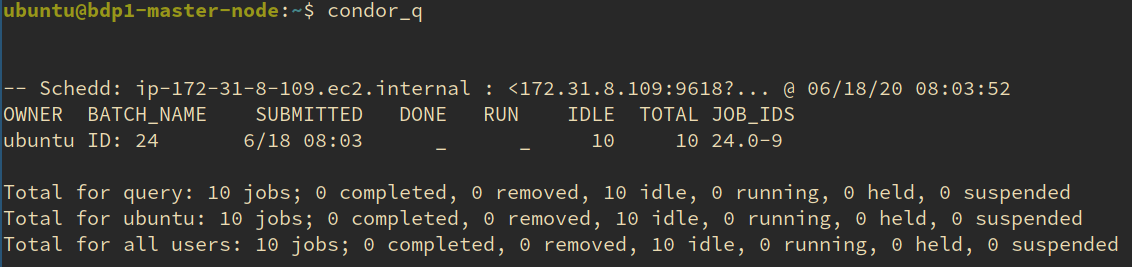
\includegraphics[width=\textwidth]{./images/condor_q.png}
    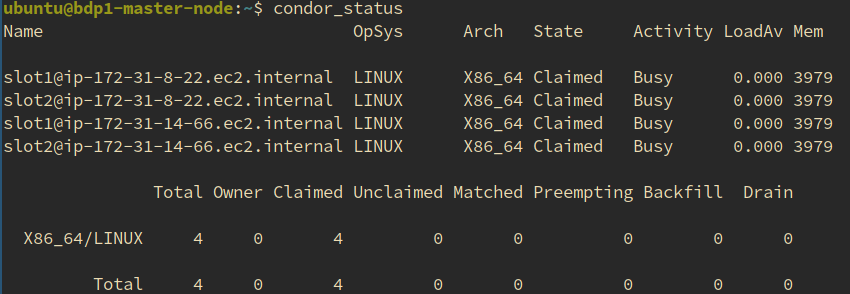
\includegraphics[width=\textwidth]{./images/condor_status_busy.png}
\end{figure}
\FloatBarrier

The cluster was able to successfully complete the task.
The test job produced the following output files:

\begin{figure}[!h]
    \center
    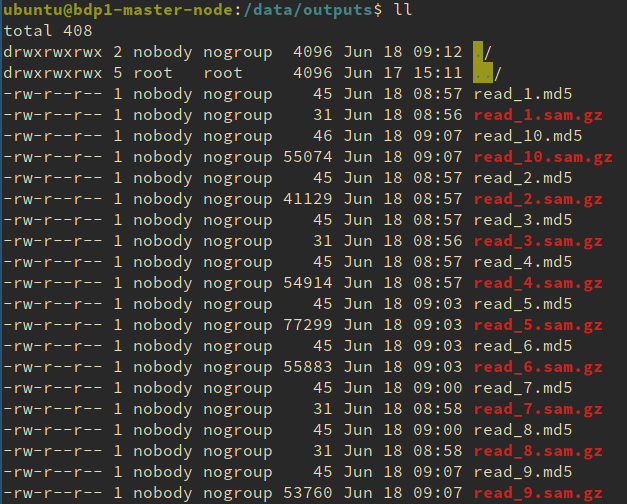
\includegraphics[width=\textwidth]{./images/condor_test_out.png}
\end{figure}
\FloatBarrier

The time required to complete the task on a single fasta file ranged from 62.77 to 422.54 seconds, with an average of 227.7 seconds.

\begin{figure}[!h]
    \center
    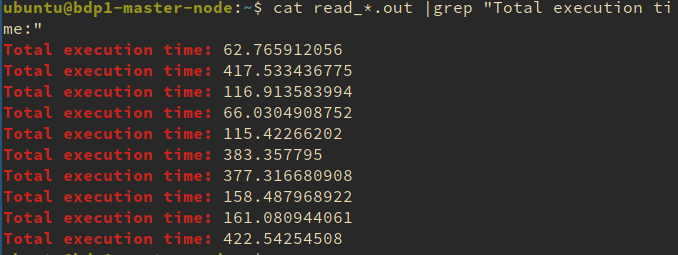
\includegraphics[width=\textwidth]{./images/time_condor.png}
\end{figure}
\FloatBarrier

\subsection{Data Management Model}
The general data management model followed was that of transferring the executables and the input fasta files using the HTCondor Input Sandbox.
Those files are generally small and their transfer is not likely to overload the Master Node.
Moreover, input data are likely to be uploaded dynamically to the cluster by users when new sequencing experiments are performed.
This approach makes the upload of new input files to the cluster more straightforward.
On the contrary, the large hg19 genome file and genome index files would be made available to the Worker Nodes through the shared NFS volume.
The Output Sandbox will contain the condor log, the standard output, and the standard error.
These files are really small and need to be immediately available to the submitter for inspecting the proceeding of the job.
The aligned reads will instead be compressed and put in the shared volume, to avoid moving large data on the Output Sandbox.

\section{Use of Docker Containers for the Task}
Docker (\texttt{https://www.docker.com/}) is a container management system that can be used to easily ship and deploy applications on a variety of platforms.
In this section I repeated the same task already accomplished, but encapsulating the BWA application in a purposes-built Docker container.
HTCondor was still used to orchestrate the execution of jobs, taking advantage of the \texttt{docker} universe.

\subsection{Configuration of the Nodes}
I created a virtual machine from the Worker Node AMI that I developped in the previous steps.
I installed Docker on it and I added the current user to the \texttt{docker} group:
\begin{lstlisting}
sudo apt install docker.io
sudo usermod -aG docker \$USER
\end{lstlisting}
I added also the user \texttt{condor} to the \texttt{docker} group:
\begin{lstlisting}
sudo usermod -aG docker condor
\end{lstlisting}

In order to make the shared NFS \texttt{/data} volume accessible to Docker containers, the file \texttt{/etc/condor/condor\_config} was modified by appending the following lines to it:
\begin{lstlisting}
# Docker configs
DOCKER_VOLUMES = BDP1_DATA
DOCKER_VOLUME_DIR_BDP1_DATA = /data
DOCKER_MOUNT_VOLUMES = BDP1_DATA
\end{lstlisting}

I created a new AMI from this virtual machine, so to be able to replicate the Worker Node instances as required by the application.
The Master Node did not need any additional configuration.

\subsection{Creation of a Containerized version of the Application}
I built a containerized version of the BWA application using \texttt{Docker}.
A container image for the BWA application was already available on DockerHub (\texttt{biocontainers/bwa}), but for educational purposes, a new image was built from scratch.
The Ubuntu Docker image was used as a base.
The Docker image \texttt{saulpierotti/bwa} was built from the following \texttt{Dockerfile} and pushed to DockerHub:

\begin{lstlisting}
FROM ubuntu
COPY ./alignment_test.py alignment_test.py
RUN chmod +x alignment_test.py
RUN apt update
RUN apt install -y bwa
RUN apt install -y python
\end{lstlisting}

The file \texttt{alignment\_test.py} mentioned in the Dockerfile was the same script used for the non-containerized version of the application.

\subsection{Execution of the Test Job}
I modified the test job file in order to use the \texttt{docker} universe instead of the \texttt{vanilla} universe.
I also added the name of to the Docker image to be used for the task (\texttt{saulpierotti/bwa}) and the path of the application executable inside the container.

\begin{lstlisting}
####################################################
############# Alignment Test Docker ################
####################################################


########### The program that will be executed #######

docker_image = saulpierotti/bwa
Executable = /alignment_test.py
readnum = $(Process)+1
arguments = read_$INT(readnum).fa

############ Input Sandbox  #########################

Input      = read_$INT(readnum).fa
transfer_input_files = read_$INT(readnum).fa

###### Output Sandbox ###############################

Log        = read_$INT(readnum).log
# will contain condor log

Output     = read_$INT(readnum).out
# will contain the standard output

Error      = read_$INT(readnum).error
# will contain the standard error

############## condor control variables #############

should_transfer_files = YES
when_to_transfer_output = ON_EXIT

Universe = docker

#####################################################

Queue 10
\end{lstlisting}

The number of Worker Nodes in the cluster was increased to 2, so to make it identical to the cluster used for the non-containerized version of the application.
The job was run on the HTCondor cluster, but after some time it was put on hold due to the exceeding of memory limits (the workers were AWS \texttt{t2.large} machines with 8 Gb of RAM).

\begin{figure}[!h]
    \center
    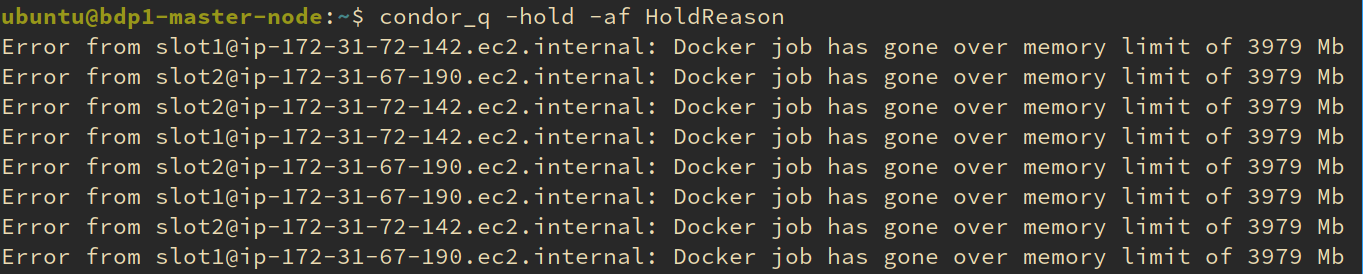
\includegraphics[width=\textwidth]{./images/docker_hold.png}
\end{figure}
\FloatBarrier

In order to solve the issue, I changed the memory reservation policy for the slots in the Worker Nodes such that 1 slot would use all the available memory, istead of sharing evenly the available memory among the 2 slots.
This was done by appending the following line to the file \texttt{/etc/condor/condor\_config}:
\begin{lstlisting}
SLOT_TYPE_1 = cpus=100%, ram=100%
NUM_SLOTS_TYPE_1 = 1
\end{lstlisting}
From the Master Node, the command \texttt{condor\_status} detected the new allocation policy:
\begin{figure}[!h]
    \center
    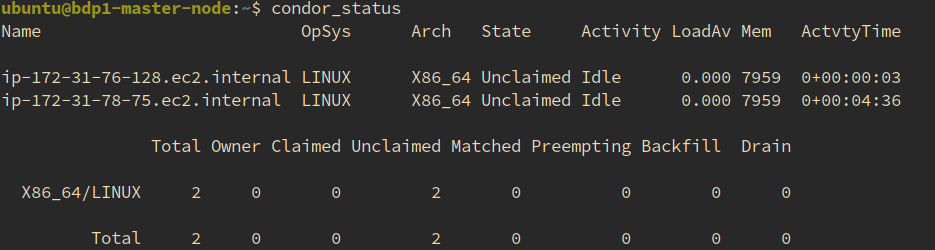
\includegraphics[width=\textwidth]{./images/condor_slot_single.png}
\end{figure}
\FloatBarrier

The job ran as planned with this new configuration.
\begin{figure}[!h]
    \center
    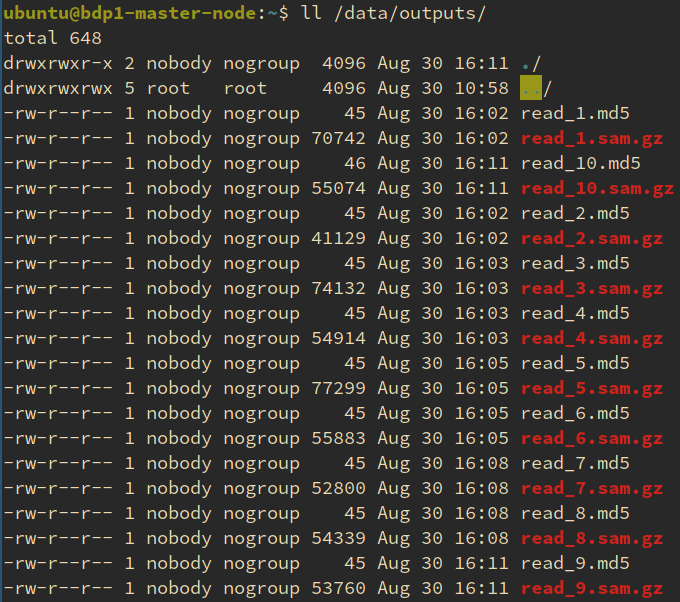
\includegraphics[width=\textwidth]{./images/condor_out_docker.png}
\end{figure}
\FloatBarrier

\subsection{Comparison of the Containerized Application with the Standard Application}
The use of Docker containers can potentially offer greater flexibility in modifying the application or its configuration.
In a traditional cluster changing the application involves creating a new AMI, terminating the worker node instances of the cluster and instanciating new worker nodes.
It would be of course possible to specify in the job description itself the packages to be installed or modified in the Worker Nodes, but this apporach is nonetheless cumbersome and could be prohibited by the administrative policies of the cluster.
With Docker containers, changing the application involves only changing the name of the Docker image to be used.
However, the main drawback of the containerized application emerged already in my small test job: increased memory requirements due to the virtualization overheads.
As seen in the previous example, in order to fulfill the increased requirements it is needed to either reduce the number of concurrent jobs that can run in the same machine (and thus reduce the performance of the cluster), or to choose a more performant (and expensive) instance type.

\section{Expected Costs}
A plausible non-trivial use-case that can be addressed using the HTCondor cluster developed in Section 1 is the alignment of a large number of fasta files deriving from a Next-Generation Sequencing (NGS) run to the human reference genome assembly hg19.

The sequencing platform manufacturer Illumina recommends aiming for a coverage of at least 30x in a human Whole-Genome Sequencing (WGS) experiment (\texttt{https://www.illumina.com/science/technology/next-generation-sequencing/plan-experiments/coverage.html}).
Given that the human genome has a size of about 3.3 billion base pairs, aiming for a 30x coverage would result in a raw output from the sequencer of at least 99 billion base pairs.
To be on the safe side, I considered a raw output of 100 billion base pairs per patient in the following cost estimate.
A single NGS read of an Illumina MySeq sequencer can have a length of up to 300 base pairs (\texttt{https://www.illumina.com/systems/sequencing-platforms/miseq.html}). Here I considered a read length of 150 base pairs, which is recommended by the manufacturer for a WGS experiment (\texttt{https://www.illumina.com/science/technology/next-generation-sequencing/plan-experiments/read-length.html}).
Under these assumptions, almost 667 million reads would need to be aligned for a single patient.
This amounts to about 667000 fasta files of 1000 reads each.

I roughly determined the time needed for aligning a fasta file containing 1000 reads of 150 base pairs each to the hg19 genome assembly in Section 1.
This corresponds to 227.3 seconds on a single core of the AWS \texttt{t2.large} machine.
Completing the alignment of the data produced in a single WGS experiment would thus require 151609100 seconds of CPU time.

The cluster described in this project consists of one Master Node and two Worker Nodes.
The Worker Nodes have two cores each, so the cluster can employ a total of four cores.
In this scenario, completing the task would require 37902275 seconds, which corresponds to more than 1 year.
Of course, this running time is not acceptable for a real-world application.
A more feasible approach would involve replicating the Worker Nodes to have more computational power.
This is possible since the alignment of a read is independent of the alignment of other reads, and so the task can be parallelized effectively.
For instance, the task could be completed in less than nine days using a cluster of 1 Master Node and 100 Worker Nodes.
This will result in a cluster with a capacity of more than 3 patients per month.
In a real use-case, the number of worker nodes in the cluster would be dimensioned relatively to the expected workload and to the maximum acceptable processing time.
The following graphs shows the number of patients that can be completely processed as a function of time in a cluster containing 2 (orange) and 100 (blue) worker nodes.

\begin{figure}[!h]
    \center
    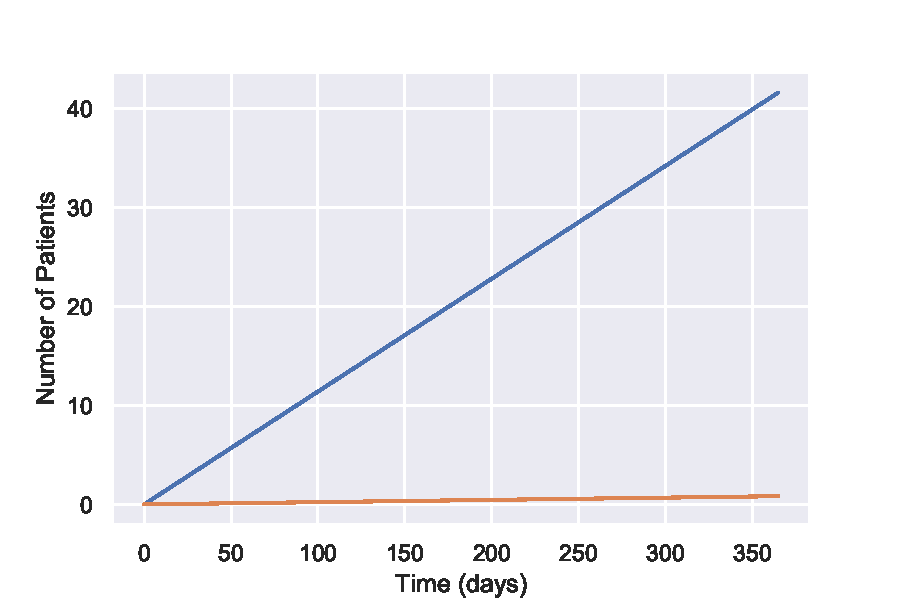
\includegraphics[width=.8\textwidth]{./images/patient_graph.pdf}
\end{figure}
\FloatBarrier

To date (May 2020) the \texttt{t2.large} machine costs \$ 0.0928 per hour, and the cluster will require 100 of them for the proposed infrastructure.
The \texttt{t2.medium} machine costs \$ 0.0464 per hour, and the cluster will require just 1 of them for the Master Node.
Storage on general-purpose SSD EBS devices costs \$ 0.1 per Gb per month.
A 1 Tb disk can be used for storing the hg19 genome and index, as well as the reads of the patients.
The following graph depicts the costs associated with running the cluster as a function of time.

\begin{figure}[!h]
    \center
    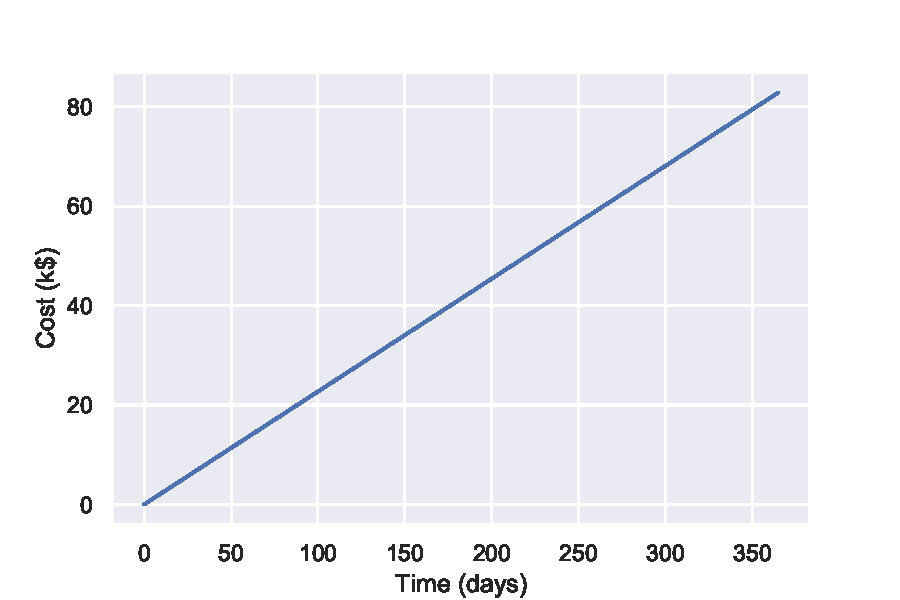
\includegraphics[width=.8\textwidth]{./images/cost_graph.pdf}
\end{figure}

\FloatBarrier

Note that costs for data movements in and out of the AWS system have been omitted.
Moreover, in a real use-case scenario, a strict security policy for dealing with medical data should be also enforced, according to local regulations.
This will likely increase the costs and the overhead required.

\section{Application of Concepts from the BDP2 Course to the Task}
In light of the topics covered in the BDP2 course, some improvements to the architecture described in this project seem possible.
For starters, it would seem reasonable to implement autoscaling of the number of worker nodes in the HTCondor cluster.
Another approach could be that of using a containerized system like a Kubernetes cluster (EKS or self-provisioned) or a Docker Swarm for running the application.
Finally, an additional possible solution is to use a serverless computing system like AWS Lambda or OpenFaaS (possibly on a self-scaling Kubernetes cluster).

Instead of using a shared NFS volume mounted on the Master Node, it could be more logical to store data on an AWS S3 bucket.
This would reduce the strain on the vital Master Node and make the data more easily accessible from outside of the cluster.

\section{References}
Li H. and Durbin R. (2009) Fast and accurate short read alignment with Burrows-Wheeler Transform. Bioinformatics, 25:1754-60. [PMID: 19451168]\\

Douglas Thain, Todd Tannenbaum, and Miron Livny, "Distributed Computing in Practice: The Condor Experience" Concurrency and Computation: Practice and Experience, Vol. 17, No. 2-4, pages 323-356, February-April, 2005.\\

Docker:\\
\texttt{https://www.docker.com/}

Recommended coverage for a WGS experiment:\\
\texttt{https://www.illumina.com/science/technology/next-generation-sequencing/plan-experiments/coverage.html}

Read lenght for a WGS experiment:\\
\texttt{https://www.illumina.com/science/technology/next-generation-sequencing/plan-experiments/read-length.html}\\
\texttt{https://www.illumina.com/systems/sequencing-platforms/miseq.html}

AWS pricing:\\
\texttt{https://aws.amazon.com/pricing}

\end{document}
